\chapter{Network Layer - Internet Protocol}
\chapterminitoc

\section{Addressing}

\subsection{Purpose and Format}

\subsubsection{Addressing in the Network Layer}

Physical addresses / MAC addresses $\rightarrow$ thường được gắn chặt với với một thiết bị (bound to a device).

$\Rightarrow$ Do đó, ta \textbf{hoàn toàn không thể} duy trì logical hierarchy (cấu trúc phân cấp logic) hay thay thế các máy chủ một cách "không gián đoạn" (in a transparent manner).
\medskip

\noindent
Logical addresses $\rightarrow$ luôn bị bắt buộc do chúng hoạt động độc lập với các thiết bị phần cứng cụ thể.

$\Rightarrow$ Việc đánh như vậy giúp tách biệt vị trí logic bên trong network khỏi physical device.

\sidebox[-3cm]{Logical address:}{
$\rightarrow$ Được sử dụng để giải quyết những limitation của MAC address trong Network Layer như:

\begin{itemize}
    \item Định tuyến và liên kết mạng (inter-networking \& routing).
    \item Xác định vị trí của thiết bị mạng trong network.
    \item Hoạt động độc lập với phần cứng.
    \item Duy trì cấu trúc phân cấp \& tính linh hoạt.
\end{itemize}
}

\begin{mybox}{Address Assignment (Cấp phát địa chỉ)}

\noindent
Với local network $\rightarrow$ việc assign một address thường không phổ biến.

\noindent
$\Rightarrow$ Hệ thống cần phải có một cơ chế tự động cấu hình địa chỉ (\textit{address autoconfiguration}).
\end{mybox}

\subsubsection{Format of IP Addresses}

\begin{itemize}
    \item \textbf{IPv4 addresses:} \begin{itemize}
        \item Độ dài: 32 bits (4 bytes) $\rightarrow$ chứa $2^{32} \approx$ 4.2 tỉ possible addresses.
        \item Sử dụng \textbf{dot-decimal notation} để biểu diễn.
        \item Ví dụ: \texttt{198.51.100.23}.
    \end{itemize}
    \item \textbf{IPv6 addresses:} \begin{itemize}
        \item Độ dài: 128 bits (16 bytes) $\rightarrow$ chứa $2^{128} = 3.4 \cdot 10^{38}$ possible addresses.
        \item Sử dụng các cụm \textbf{hexadectets/quad-nibbles} (cụm 4 số thập lục phân) được phân tách thành các dấu hai chấm (colons).
        \item Ví dụ: \texttt{2001:0db8:0000:0000:0000:ff00:0042:8329} (hoặc viết gọn: \texttt{2001:db8::ff00:42:8329}).
    \end{itemize}
\end{itemize}

\begin{mybox}{Address Space}
\noindent
Là tổng số lượng \textbf{tất cả} các mã định danh mạng hợp lệ (valid network identifiers).
\end{mybox}

\section{Address Resolution}

\subsection{Address Resolution}

\begin{figure}[H]
    \centering
    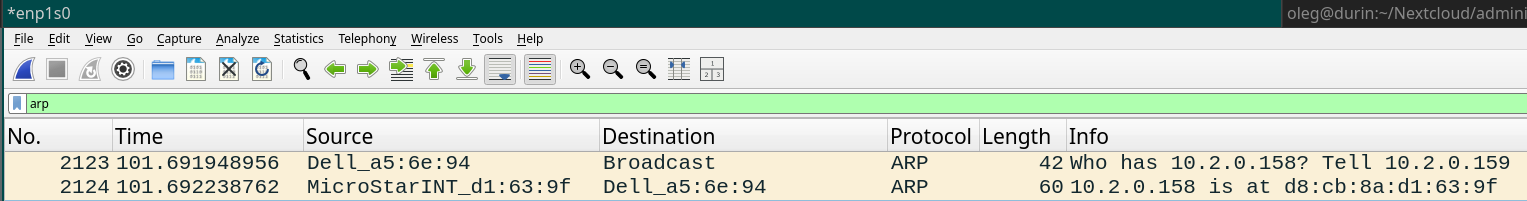
\includegraphics[width=1\textwidth]{assets/chap_5/addr_resolution.png}
\end{figure}
\medskip

\noindent
Network Layer yêu cầu việc ánh xạ (mapping) giữa các physical network address (ví dụ như MAC) và logic network address (ví dụ như IP) để có thể truyền dữ liệu thành công.
\medskip

\subsection{IPv4: Address Resolution Protocol (ARP)}

\noindent
\textbf{ARP} được sử dụng để phân giải từ \textbf{IPv4 address} sang MAC address.
\medskip

\sidebox{Address Resolution Protocol (ARP):}{
Là giao thức \textbf{phân giải địa chỉ}.

\noindent
$\Rightarrow$ Dùng để tìm (phân giải) physical MAC address của một thiết bị mạng khi đã biết trước logic address của nó.
\medskip

\noindent
\textit{*ARP chỉ áp dụng trong IPv4.}
}

\noindent
\textbf{Cách ARP vận hành:}

\begin{figure}[H]
    \centering
    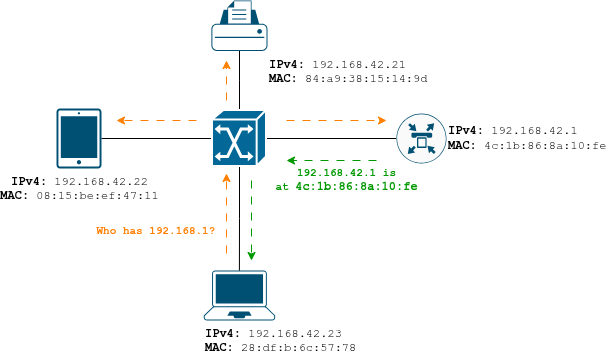
\includegraphics[width=1\textwidth]{assets/chap_5/arp_simplify.png}
\end{figure}

\sidebox[1cm]{Note:}{ARP sử dụng \textbf{broadcast messages}.}

\begin{enumerate}
    \item \textbf{Gửi yêu cầu:} gửi MAC broadcast frame chứa địa chỉ IP của thiết bị cần tìm đến trong mạng LAN.
    \item \textbf{Kiểm tra:} mỗi thiết bị nhận được frame này sẽ lấy IP address bên trong để đối chiếu với IP của mình.
    \item \textbf{Phản hồi:} thiết bị nào có IP trùng khớp thì sẽ gửi unicast response trực tiếp cho máy gửi ban đầu, trong đó có chứa MAC address của nó.
    \item \textbf{Ánh xạ:} máy sẽ map địa chỉ MAC vừa nhận được với địa chỉ IP mà nó đang tìm kiếp để tiến hành truyền dữ liệu.
\end{enumerate}
\medskip

\subsection{IPv6: Neighbor Discovery Protocol (NDP)}

\noindent
\textbf{NDP} đảm nhận vai trò tương tự như ARP nhưng dành cho mạng \textbf{IPv6}.
\medskip

\sidebox{Neighbor Discovery Protocol (NDP):}{
Là giao thức "khám phá láng giềng" $\rightarrow$ phân giải địa chỉ để mapping giữa logic address (IPv6) và physical address (MAC).
\medskip

\noindent
\textit{*NDP chỉ áp dụng trong IPv6.}
}

\noindent
\textbf{Cách NDP vận hành:}

\begin{figure}[H]
    \centering
    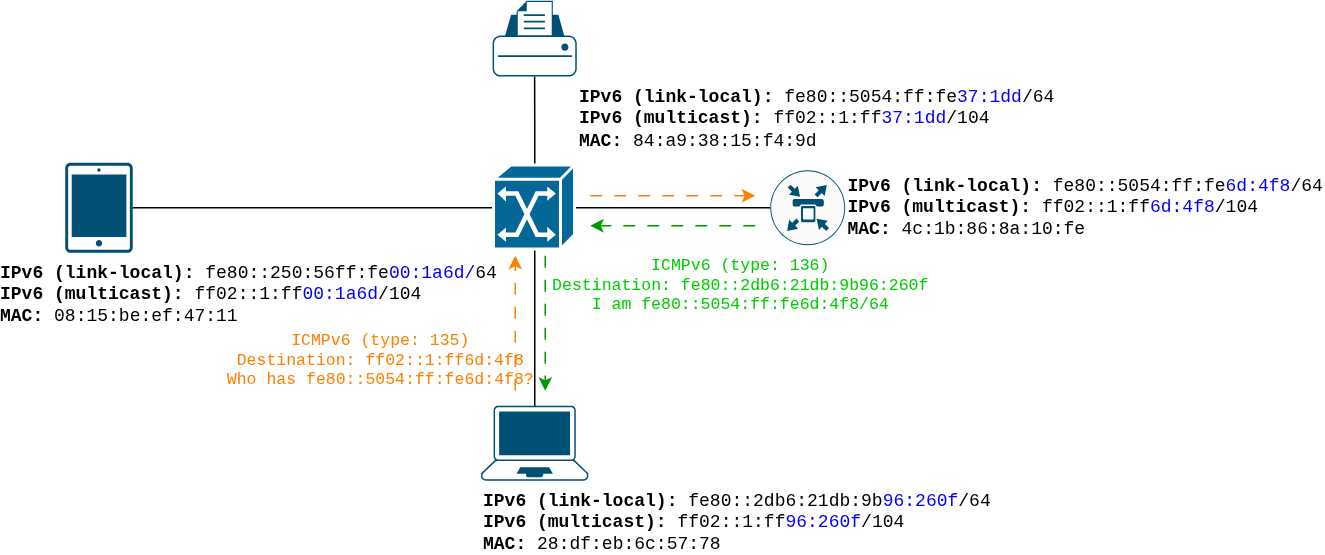
\includegraphics[width=1\textwidth]{assets/chap_5/ndp_simplify.png}
\end{figure}

\sidebox[1cm]{Note:}{NDP sử dụng \textbf{multicast messages}.}

\begin{enumerate}
    \item \textbf{Solicited-node multicast address:} giao thức này sử dụng một destination address đặc biệt có prefix là \texttt{ff02::1:ff00:0000/104}; 24 bits còn lại được lấy từ 24 bits cuối của unicast address tương ứng với thiết bị.
    \item \textbf{Đăng kí nhóm multicast address:} mỗi node sẽ tự động đăng kí tham gia vào nhóm multicast này cho từng unicast address được config $\rightarrow$ chỉ những node nào có đăng kí address này thì mới nhận và xử lý các tin nhắn ICMP tương ứng (ví dụ: \textit{Type 135} cho yêu cầu, \textit{Type 136} cho phản hồi) $\Rightarrow$ giảm tải cho các thiết bị không liên quan trong mạng.
    \item \textbf{Giao tiếp linh hoạt:} các routers và các nodes có thể chủ động phát đi các advertisements (tin nhắn thông báo) hoặc phản hồi lại các truy vấn thông qua yêu cầu từ router và neighbor solicitations (truy vấn láng giềng).
\end{enumerate}
\medskip

\sidebox[-3cm]{Internet Control Message Protocol (ICMP):}{
Được sử dụng chủ yếu để trao đổi tin nhắn chẩn đoán (diagnostic), điều khiển \& báo lỗi (error messages) trong hệ thống mạng.

\noindent
$\Rightarrow$ Tất cả các routers và terminal devices (thiết bị đầu cuối) đều có khả năng xử lý giao thức này.
}

\subsection{Neighbor Cache}

\noindent
\textbf{Neighbor cache} (bộ nhớ đệm láng giềng) $\rightarrow$ sử dụng để làm \textbf{tăng tốc độ phân giải địa chỉ} (speed up the address resolution).
\medskip

\noindent
$\Rightarrow$ Chứa một bảng lưu trữ các thông tin cho mỗi entry (bản ghi) gồm:

\begin{itemize}
    \item Layer 3 protocol type (như IPv4).
    \item Layer 3 address (như IP address).
    \item Layer 2 address (MAC address).
\end{itemize}
\medskip

\begin{mybox}{Tips}
\noindent
Command để hiển thị neighbor cache trên máy: \textbf{\texttt{arp -n}} hoặc \textbf{\texttt{ip neighbour}}.
\end{mybox}
\medskip

\begin{verbatim}
# arp -n
Address         HWtype  HWaddress          Flags Mask  Iface
192.168.178.1   ether   9c:c7:a6:b9:32:aa  C           wlan0
192.168.178.24  ether   d4:85:64:3b:9f:65  C           wlan0
192.168.178.41  ether   ec:1f:72:70:08:25  C           wlan0
192.168.178.25  ether   cc:3a:61:d3:b3:bc  C           wlan0
\end{verbatim}
\medskip

\section{IPv4 Networks}

\subsection{Network Identifier and Host Identifier}

\noindent
32 bits của IPv4 address được chia thành 2 phần:

\begin{itemize}
    \item \textbf{Network identifier} (mã định danh mạng, còn gọi là network ID): dùng để xác định mạng lưới đang kết nối vào $\rightarrow$ tất cả các thiết bị (host) \textbf{kết nối vào cùng một mạng} thì sẽ \textbf{bắt buộc phải có chung phần network ID} này.
    \item \textbf{Host identifier} (mã định danh thiết bị, còn gọi là host ID): dùng để xác định một thiết bị cụ thể nằm bên trong network đó.
\end{itemize}
\medskip

\noindent
$\rightarrow$ Số lượng bits dành cho \textit{network ID} và \textit{host ID} \textbf{có thể thay đổi} theo nhu cầu chứ không cố định.
\medskip

\begin{mybox}{Nguyên lý phân bổ số bits cho Network ID}
\noindent
Nếu mạng dùng \textbf{ít bits} cho phần network ID $\rightarrow$ \textbf{bits còn lại} cho phần host ID sẽ \textbf{nhiều lên} $\Rightarrow$ mạng đó sẽ chứa được \textbf{nhiều thiết bị kết nối} hơn.
\end{mybox}
\medskip

\sidebox[-3cm]{Self-note:}{
Độ dài của IPv4 nó luôn 32 bits, nên là nếu host ID chiếm nhiều bit hơn $\rightarrow$ sẽ cho nhiều connection hơn. 
\medskip

\noindent
Tương tự như network ID.
}
